\chapter{RESULTADOS}
\label{chp:results}

Este capítulo apresenta os resultados dos três experimentos descritos no capítulo \ref{chp:experiments}. Os resultados serão divididos em três seções, uma para cada experimento.

\section{Experimento 1} 
\label{sec:results:experiment-1}

Conforme descrito no capítulo \ref{chp:experiments}, este experimento utiliza 100 pares código-fonte/comentário da base de treinamento para determinar a capacidade semântica do modelo de comparação, através da remoção de palavras aleatórias do comentário.

A Figura \ref{fig:experiment-1:good} apresenta um resultado positivo de um dos 100 pares utilizados.
\begin{figure}[H]
  \centering
    \caption{Exemplo de resultado positivo}
    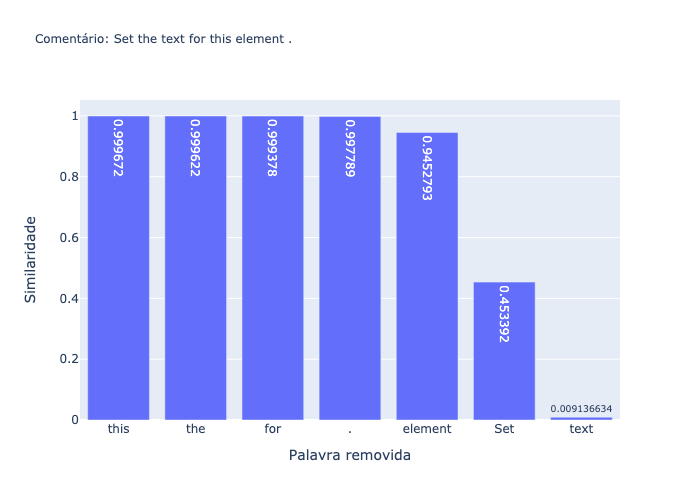
\includegraphics[scale=0.6]{imagens/resultados/experiment-1/sample_5.png}
    \smallcaption{Fonte: Autor}
    \label{fig:experiment-1:good}
\end{figure}

Na Figura \ref{fig:experiment-1:good}, gráfico mostra o comentário do par selecionado, a palavra removida (eixo x) e a similaridade (eixo y) obtida pelo modelo de comparação. Vale lembrar que ao remover uma palavra do comentário, obtem-se a \textit{query} $C^-$. Isso significa que, usando os dados da Figura \ref{fig:experiment-1:good} como exemplo, dado que o comentário é \textit{Set the text for this element.}, ao remover a palavra \textit{this}, obteve-se a \textit{query} $C^-$ \textit{Set the text for element.}.

Vale lembrar que o modelo de comparação foi treinado utilizando como entrada os \textit{embeddings} de código-fonte e do seu respectivo comentário. Portanto, valores de similaridade altos neste experimento indicam que o modelo não considerou a palavra removida importante para a busca; de igual modo, similaridade baixa indica que a palavra removida era importante para o par em questão.

O resultado da Figura \ref{fig:experiment-1:good} é considerado positivo pois, ao se retirar palavras menos relevantes do comentário, a similaridade se manteve alta - como se tivéssemos utilizado o próprio comentário como \textit{query}. De igual modo, quando palavras relevantes foram removidas, a similaridade diminuiu como pode-se notar nas similaridades das palavras \textit{text} e \textit{Set}.

Outro ponto interessante desse resultado é notar que o modelo conseguiu captar informações semânticas do comentário. A Figura \ref{fig:experiment-1-medium} mostra o par código-fonte/comentário em questão.

\begin{figure}[H]
  \centering
    \caption{Exemplo de resultado positivo}
    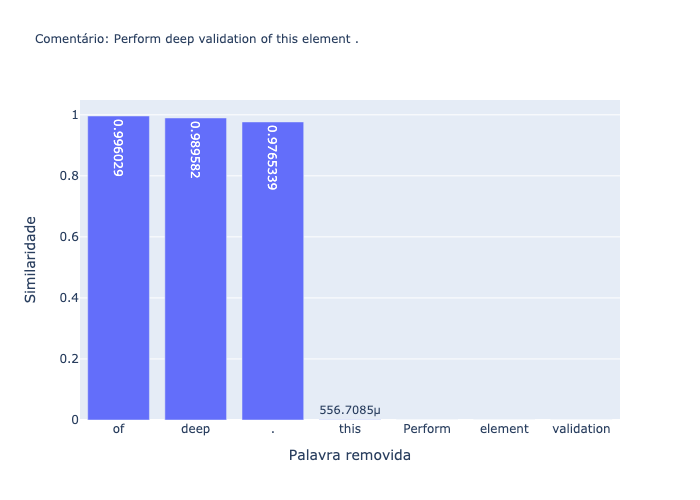
\includegraphics[scale=0.6]{imagens/resultados/experiment-1/sample_9.png}
    \smallcaption{Fonte: Autor}
  \label{fig:experiment-1-medium}
\end{figure}

A Figura \ref{fig:experiment-1-medium} mostra que o trecho de código-fonte em questão é responsável por atribuir (\textit{set}) dada palavra, chamada pelo autor do código de \textit{text}, ao valor de \textit{TextContent}. Com isso, as palavras \textit{text}, \textit{set} e \textit{content} são semanticamente importantes nesse par, o que corrobora os resultados apresentados na Figura \ref{fig:experiment-1:good}.

Em outro par, o modelo acertou a maioria das palavras relevantes, conforme apresentado na Figura \ref{fig:experiment-1-medium}.

Os resultados do modelo mostram que, para o comentário \textit{Perform deep validation of this element.}, as palavras \textit{validation}, \textit{element} e \textit{Perform} são semanticamente relevante para o par em questão, o que é verdade. Entretanto, o modelo também considerou relevante a palavra \textit{this}, e não considerou importante a palavra \textit{deep} o que, dado o contexto, seria exatamente ao contrário: \textit{this} deveria ser significativamente menos relevante do que \textit{deep}.

Por fim, a Figura \ref{fig:experiment-1-bad} apresenta um par onde o modelo não conseguiu detectar o significado semântico das palavras do comentário.

\begin{figure}[H]
  \centering
    \caption{Exemplo de resultado negativo}
    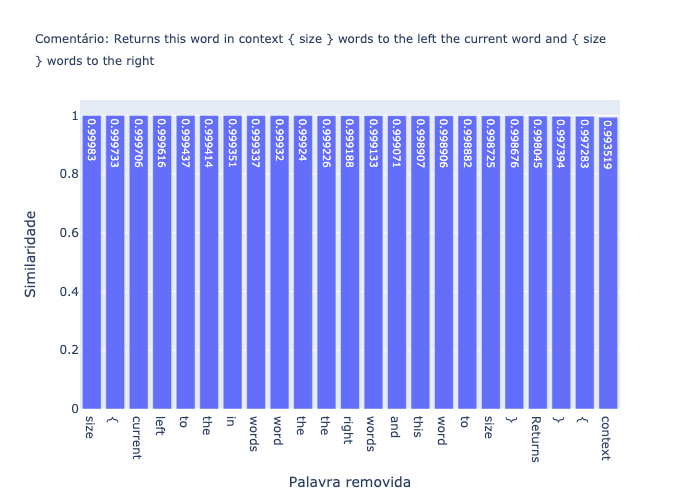
\includegraphics[scale=0.65]{imagens/resultados/experiment-1/sample_29.png}
    \smallcaption{Fonte: Autor}
    \label{fig:experiment-1-bad}
\end{figure}

Na Figura \ref{fig:experiment-1-bad} é possível ver que todas as palavras retiradas obtiveram valores muito próximos de similaridade, o que representa que o modelo de comparação não conseguiu determinar quais palavras eram semanticamente relevantes para o par em questão. Além disso, verificou-se nesse experimento que, quando o par possui comentário com 20 palavras ou mais, esses resultados geralmente se repetem, ou seja, o modelo não consegue determinar quais palavras são mais relevantes para o par em questão. Uma possível explicação seja que, dado o tamanho do comentário e do código-fonte, o modelo não consiga extrair informações sobre o contexto do par e, portanto, não consegue determinar as palavras mais relevantes.

Por fim, 100 pares código-fonte/comentário foram utilizados durante este experimento, gerando 1439 $C^-$, com tempo de execução de 1 minuto e 40 segundos.

\section{Experimento 2} 
\label{sec:results:experiment-2}
O objetivo desse experimento é determinar a performance do modelo de comparação na tarefa de busca de código-fonte a partir de linguagem natural. Para tanto, utilizou-se as mesmas 100 pares código-fonte/comentário do experimento 1, além das métricas de recuperação de informação \gls{mrr} e \textit{SuccessRate@k} com $k=1$, $k=5$ e $k=10$. Foi aplicado o mesmo processo de geração de \textit{queries} $C^-$ utilizado no experimento 1. Portanto, para cada par, realizou-se uma busca de código-fonte para cada uma das \textit{queries} $C^-$ geradas. 

Aqui, da lista de resultados resultante de cada busca, considera-se que o código-fonte do par em questão é o mais relevante. Portanto, ao se fazer uma busca utilizando a \textit{query} $C^-$ gerada a partir do comentário do $par_i$, o código-fonte mais relevante da lista de resultados será o código-fonte do mesmo $par_i$. Inclusive, a posição desse código-fonte na lista de resultados será utilizada para calcular as métricas \gls{mrr} e \textit{SuccessRate@k}.

Portanto, a Figura \ref{fig:experiment-2-mrr} mostra os valores de \gls{mrr} para cada um dos 100 pares utilizados. Neste experimento, o menor valor de \gls{mrr} foi de $0.008$ enquanto o maior foi de $0.783$. Ainda, a média de todos os valores obtidos de \gls{mrr} foi de aproximadamente $0.130$.

\begin{figure}[H]
  \centering
      \caption{\textit{MRR}}
      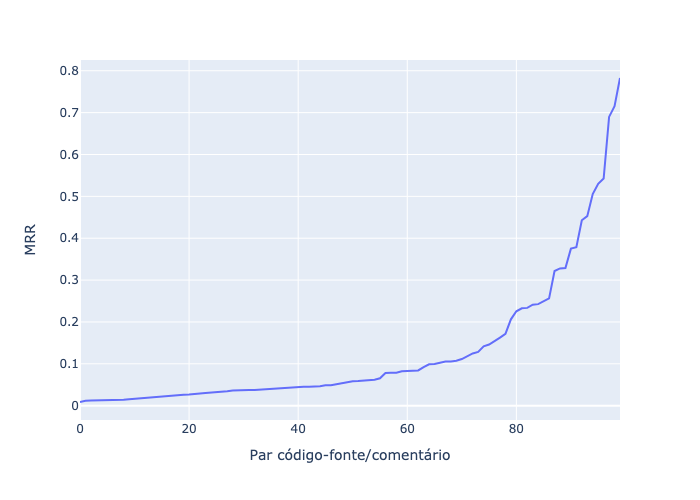
\includegraphics[scale=0.6]{imagens/resultados/experiment-2/mrr.png}
      \smallcaption{Fonte: Autor}
      \label{fig:experiment-2-mrr}
\end{figure}


Em relação ao \textit{SuccessRate@k}, a Figura \ref{fig:experiment-2-success-k} mostra os resultados obtidos para $k=1$, $k=5$ e $k=10$. Com esses valores de $k$, os maiores resultados obtidos foram de $0.933$, $0.960$ e $1.000$, respectivamente, enquanto o menor resultado foi zero para todos os valores de $k$. A média dos resultados foi de, aproximadamente, $0.044$, $0.176$, $0.297$ para os valores de $k=1$, $k=5$ e $k=10$, respectivamente.

\begin{figure}[H]
  \centering
      \caption{\textit{SuccessRate@k}}
      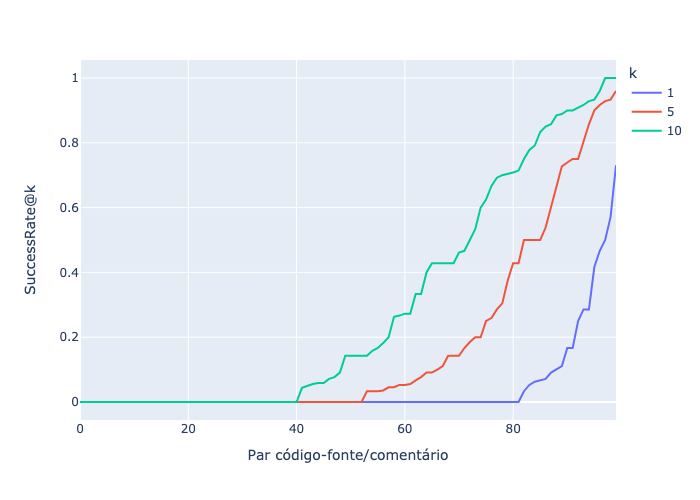
\includegraphics[scale=0.6]{imagens/resultados/experiment-2/success-rates.png}
      \smallcaption{Fonte: Autor}
      \label{fig:experiment-2-success-k}
\end{figure}

Por fim, o tempo total de execução desse experimento foi de 27 minutos e 55 segundos.

\section{Experimento 3} 
\label{sec:results:experiment-3}
Por fim, o experimento 3 utiliza as \textit{queries} $Q_{cs}$ da base de dados \textit{CodeSearchNet}, bem como os valores esperados para cada \textit{query} $Q_{cs}$, também contidos na base \textit{CodeSearchNet}, para determinar a quantidade de acertos do modelo de comparação utilizando os dados contidos na base em questão. O objetivo é determinar a performance do modelo de comparação proposto neste estudo com o padrão estabelecido pelos autores da base \textit{CodeSearchNet}. Este valor é chamado pelos autores de relevância.

Para determinar se o modelo obteve o valor correto em relação ao esperado para determinada \textit{query}, foi realizado uma normalização do valor de similaridade em relação ao valor esperado. Com isso, espera-se que valores de similaridade iguais ou menores que $0.5$ possuam relevância de 0 ou 1, enquanto valores de similaridade maiores que $0.5$ tenham relevância igual a 2 ou 3, conforme descrito na seção \ref{sec:experiments:experiment-3}.

Portanto, utilizando os parâmetros contidos na base de dados \textit{CodeSearchNet} \cite{Husain2019CodeSearchNetCE}, o modelo de comparação obteve $54.99\%$ de acerto, com 463 predições corretas de 842 \textit{queries}. Além disso, o tempo de execução do experimento em questão foi de $13.6$ segundos.

